\section{\repbox Background} \label{sec:background}

\repbox's deployment is similar to a typical \smr's. In a \repbox-replicated
system, a set of 2\v{f}+1 machines (nodes) are set up within a LAN,
and each node runs an instance of \repbox containing the same server
program. Once the \repbox system starts, one node becomes the \emph{primary}
node which proposes the order of requests to execute, and the others
become backup nodes which follow the primary's proposals. An arbitrary
number of clients in LAN or WAN send network requests to the primary and
get responses.  If failures occur, the nodes run a leader election to
elect a new leader and continue. Despite \v{f} nodes fail, \repbox still 
guaratees availability of the replicated application.

Figure~\ref{fig:repbox} shows an instance of \repbox running on 
each node. This section presents the background of \repbox's two key techniques, 
\smr (\S\ref{sec:smr}) and \dmt (\S\ref{sec:dmt}).

\begin{figure}[t]
\vspace{.20in}
\centering
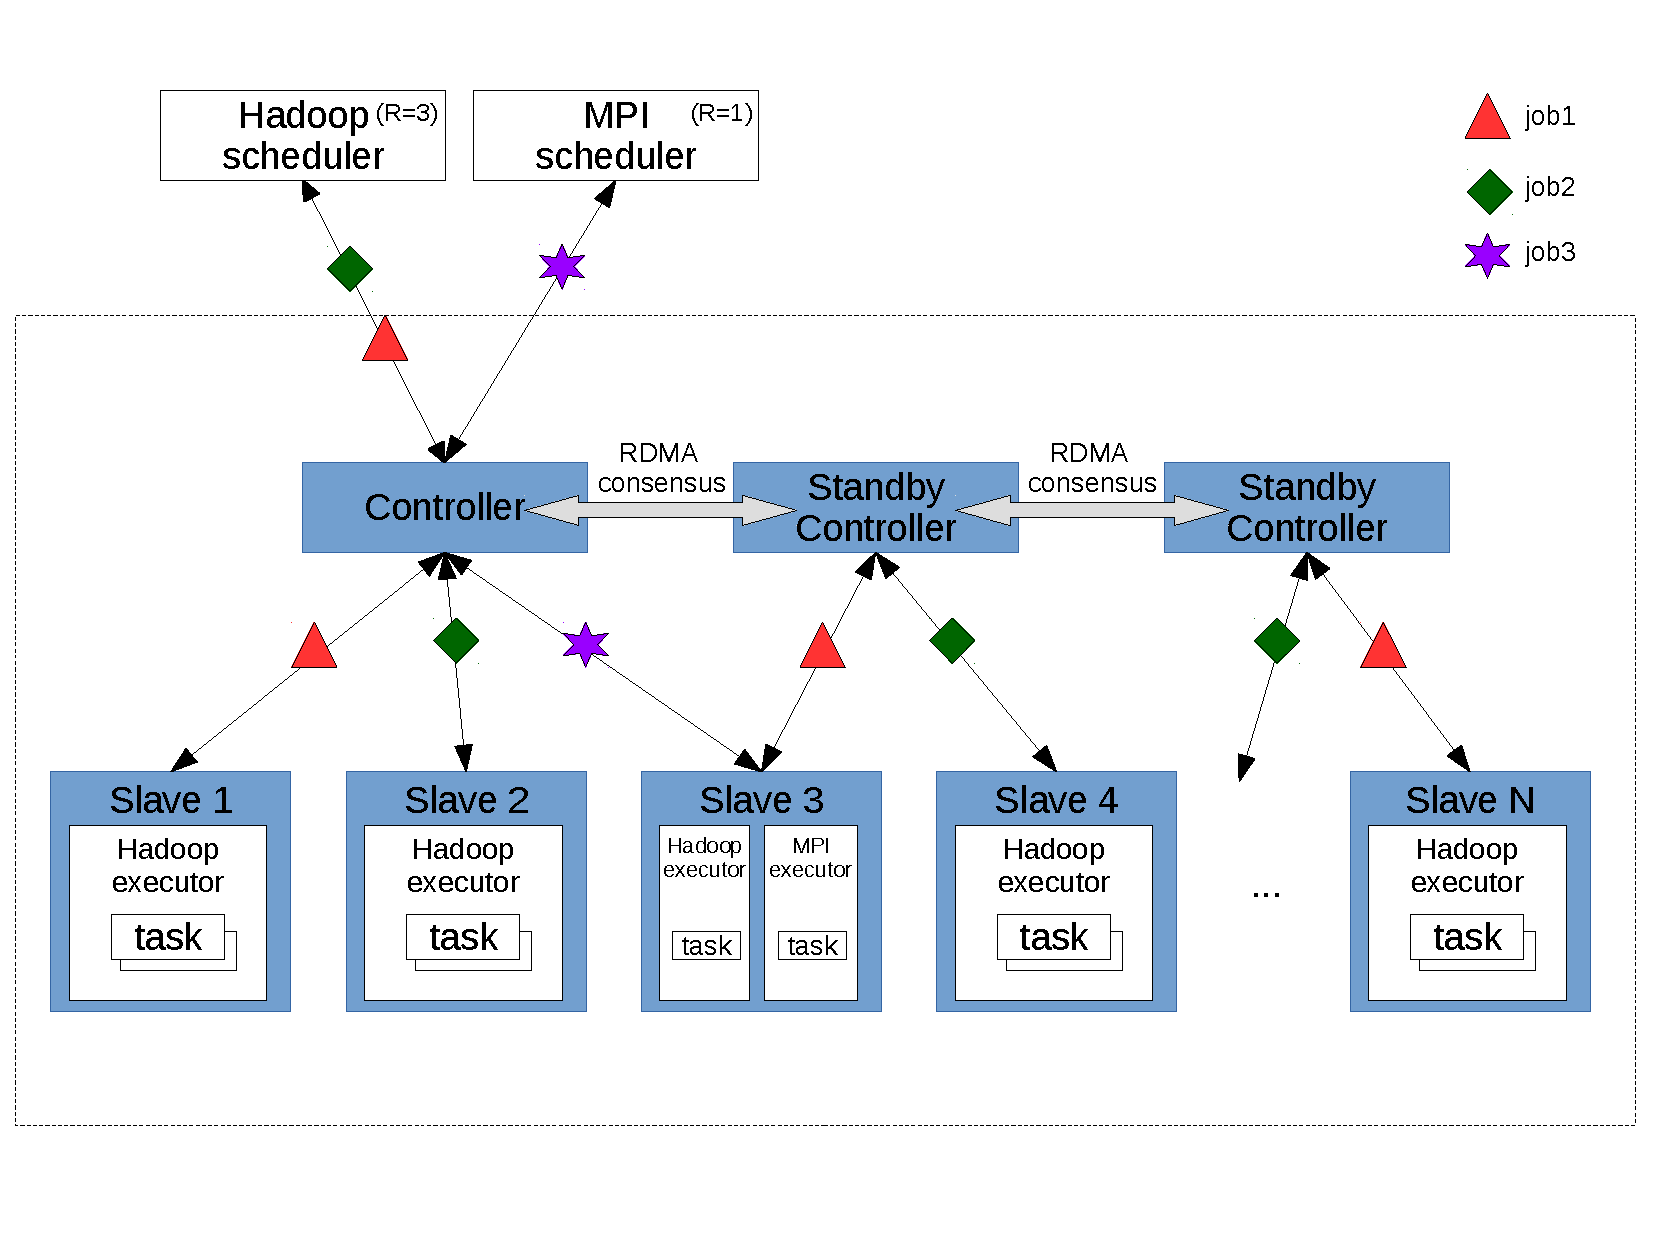
\includegraphics[width=.5\textwidth]{figures/arch}
\vspace{-.20in}
\caption{{\em The \repbox Architecture.} \repbox components are shaded (and in
  green).} \label{fig:repbox}
\vspace{-.05in}
\end{figure}


\subsection{State Machine Replication (\smr)} \label{sec:smr}

State machine replication (\smr) is a powerful fault-tolerance
concept~\cite{paxos:practical}.  It models a program as a deterministic state 
machine, where states are important program data and the transitions are 
deterministic executions of program code under input requests.  \smr runs 
replicas of this state machine on multiple nodes, tolerating many possible node 
and network failures.  To keep the replicas consistent, it invokes a
distributed consensus protocol (typically \paxos~\cite{paxos, paxos:simple, 
paxos:practical}) to ensure that a quorum (typically majority) of the replicas 
agree on the input request sequence; under the deterministic execution 
assumption, this quorum of replicas must reach the same exact state.  \smr is 
proven safe in theory, and provides high availability in practice.

To support general server programs transparently, \repbox leverages \repbox's 
\paxos consensus protocol, which takes the POSIX socket API as
consensus interface. This \paxos protocol enforces two kinds of 
orders for socket operations. First, for requests coming from the clients, 
such as \connect and \send requests, this protocol enforces that all nodes see 
the same totally ordered sequence of these requests using the \paxos and socket 
API interposition components.  (this protocol does not need to order the 
blocking socket operations in the clients because we mainly focus on analyses 
for server applications.) Second, for server applications' blocking operations, 
this \paxos protocol schedules them according to the matching operations from 
the clients (\eg, a \send from a client matches a \recv from the server within 
the same socket connection). This protocol does not schedule non-blocking 
operations in servers (\eg, \send to clients) because it focuses on replicating 
the server's execution states.

For practicality, \repbox's \paxos implementation takes a well-known 
engineering approach~\cite{paxos:practical}: only the primary invokes consensus 
request during normal operations, and an leader election is invoked when 
exceptions such as network partitions occur.


In a \repbox instance, the \paxos consensus component is the gateway.  This 
component accepts socket requests from the clients and invoke a \paxos 
consensus instance with the other replicas on this operation. Once a consensus 
is reached, this component forwards the operation to the \dmt component. This 
component is also the only \repbox component that communicates among different 
\repbox instances. 

In this paper, \xxx skips the fault-tolerance nature of \repbox, but leverages it 
to construct multiple equivalent executions for analysis tools.

\subsection{Deterministic Multithreading (\dmt)} \label{sec:dmt}

\dmt~\cite{dpj:oopsla09, 
dmp:asplos09, kendo:asplos09, coredet:asplos10, dos:osdi10, ddos:asplos13, 
ics:oopsla13} is an advanced threading technique that enforces the same 
schedule 
on the same inputs.  This technique typically maintains a \emph{logical
  time}\footnote{Though related, the logical time in \dmt is not to be
  confused with the logical time in distributed
  systems~\cite{lamportclock}.} that advances deterministically based on
the code run.  It allows a thread to synchronize only at deterministic
logical times.  By induction, it makes an entire multithreaded execution
deterministic.  The overhead of \dmt is typically moderate: one recent
\dmt system, \parrot~\cite{parrot:sosp13}, incurs an average of 12.7\%
overhead on a wide range of 108 popular multithreaded programs on 24-core
machines.

The \dmt component runs within the same process as a server replica, and
enforces the same logical clocks for inter-thread communication
operations. \repbox leverages the \parrot~\cite{parrot:sosp13} \dmt runtime
system because it is fast (\ie, 12.7\% overhead for a wide range of 108 popular 
multithreaded programs) and transparent to the application.


Specifically, \parrot uses a runtime technique called \ldpreload to dynamically 
intercept \pthread synchronizations (\eg, \mutexlock) issued by an executable 
and enforces a well-define, round-robin schedule on these synchronization 
operations for all threads, practically eliminating nondeterminism in thread
synchronizations. Although \parrot is not designed to resolve data races
deterministically, deploying a race detector in one replica can overcome this 
limitation (\S\ref{sec:discuss}).  \repbox augments the \dmt component to schedule 
the return points of blocking socket operations in server replicas, too, to 
ensure that requests are admitted exactly at the same logical time across 
replicas.



% Our model. Multiple writer multiple reader.
\section{\xxx Overview} \label{sec:model}

\xxx's main purpose is to support transparent analyses, so its deployment model is different 
from \repbox's: in \xxx, a set of 2\v{f}+1 
machines (for short, nodes) are set up within a LAN. Among these nodes, at 
least \v{f}+1 nodes run an actual execution or a lightweight analysis tool on 
each so that they can reach consensus on inputs and process requests fast, 
while at most \v{f} nodes run an heavyweight analysis tool on each. Once the 
\xxx system starts, one node becomes the \emph{primary} node which proposes the 
order of requests to execute, and the other nodes become backup nodes which 
follow the primary's proposals. An arbitrary number of clients in LAN or WAN 
send network requests to the primary and get responses.

TBD: emphasis what is lightweight and heavyweight. Suggestions.

Figure~\ref{fig:arch} shows an instance of \xxx running on 
each node. The instance contains three main components, the \paxos consensus 
component, the \dmt scheduler, and the checkpointer component. A server program 
runs transparently in a \xxx instance with or without an analysis tool. Neither 
the server or the analysis is aware of \xxx's components.




\subsection{Discussion} \label{sec:discuss}

\subsubsection{What Types of Analyses are Suitable to Run in \xxx?} 
\label{sec:analysis-types}

We envision that an analysis can transparently run in \xxx if: (1) it can run 
asynchronously with the actual execution, and (2) it does not schedule 
conflicting order of \pthread synchronizations that \xxx's \dmt runtime 
enforces. Many reliability analyses (\eg, data race detection), profiling, 
and logging tools meet this requirement.

Some synchronous security analysis such as control 
flow integrity can not transparently run in \xxx because it monitors the 
execution 
synchronously for each control flow transfer. In addition, some other security 
analysis such as information leakage protection can not transparently run in 
\xxx 
because the actual execution may probably run faster than the 
analysis and leak information to clients before the analysis detects the 
leakage. Nevertheless, many security tools such as use-after-free 
vulnerabilities can be transparently deployed in \xxx. If a synchronous 
analysis 
tool would like to run in \xxx, it should use \xxx's checkpoint 
and rollback APIs (\S\ref{sec:checkpoint}).


\subsubsection{Can \xxx Strengthen Existing Analyses?} 
\label{sec:strengthen-analysis}

\xxx has the potential to strengthen existing analyses via its performance 
benefit. Previously, to mitigate the huge performance slowdown, some analysis 
tool developers sometimes have to weaken the guarantees of an analysis. For 
instance, ThreadSanitizer\cite{tsan}, one of the most practical race detectors, 
only logs the last four accesses for each memory byte instead of the complete 
access history, because logging and analyzing the complete history is quite 
heavyweight (\eg, 20X+ slowdown for some testing programs the authors 
evaluated). However, an incomplete access history may miss data races at 
runtime. With \xxx, developers can now strengthen the analysis by logging 
complete memory access history.

\xxx also has the potential to speedup existing analysis tools themselves via 
its replication architecture. For instance, the high logging overhead for 
failure reproductions on multi-processors is an open research 
problem~\cite{sherlog:asplos10}. Fortunately, with \xxx's architecture, these 
logging tools now can separate different logging aspects such as functions, 
libraries, and threads into different replicas (\eg, each replica logs for only 
one thread), greatly reducing the logging overhead. Sampling-based race 
detection tools (\eg,~\cite{datacollider:osdi10}) can also greatly reduce 
sampling overhead by dividing sampling work into replicas, or can significantly 
multiply sampling rates by running the same tool among replicas.

Moreover, \xxx provides an extra fault-tolerance benefit for analysis tools. 
Existing reliability and security analyses tend to expose or detect harmful 
defeats in an application, which may crash the application. In addition, the 
actual executions across different nodes may fail as well due to hardware or OS 
failures. With \xxx's \smr architecture, the sequence of inputs are 
persistently and consistently enforced across replicas, and failing minor 
nodes (either an analysis or an actual execution node) do not affect the other 
nodes' executions and analyses.

% \subsection{Can \xxx Speedup Existing Analyses?} 
% \label{sec:speedup-analysis}
% 
% TBD.

\subsubsection{Can Existing Analyses Benefit \xxx?} 
\label{sec:strengthen-crane}

Interestingly, analyses running in \xxx can benefit \xxx's \dmt runtime and 
improve \xxx's performance. Existing typical \dmt systems use two approaches to 
enforce schedules. First, a \dmt approach enforcing a total order order for 
shared memory accesses (for short, mem-schedules) is fully deterministic even 
with data races, but this approach incurs prohibitive slowdown. For instance, 
\dthreads~\cite{dthreads:sosp11} incurs several times slowdown for many 
programs because typical applications have intensive amounts of shared memory 
accesses.

The other \dmt approach is enforcing a total order for 
synchronizations only (for short, sync-schedules). This approach can be 
efficient because most code is not synchronization and can still run in 
parallel. For instance, \kendo, \tern, and \peregrine~\cite{kendo:asplos09, 
cui:tern:osdi10, parrot:sosp13} incurred less than 16\% overhead on most 
programs they evaluated. However, this approach is only deterministic when 
no races occur. Overall, despite much effort~\cite{dthreads:sosp11, 
parrot:sosp13, peregrine:sosp11, determinator:osdi10}, an open problem still 
exists: people lack a simple and deployable approach to enforce fully 
deterministic and efficient \dmt schedules.


Fortunately, \xxx's replication architecture can address this problem by simply
running a race detector in one replica, then \xxx can choose the faster \dmt 
approach that enforces sync-schedules. If the race detector reports a race, 
application developers can easily diagnose and fix it because synchronization 
schedules enforced by \dmt already make races easily 
reproducible~\cite{pres:sosp09}. By enforcing the same synchronization 
schedules across replicas, race detection results consistently hold for all 
replicas. In sum, \xxx and race detection tools form a mutually beneficial 
eco-system.
